\chapter{Excommunication}

When someone goes against the church's teachings and openly oppose the church and its
leaders, they can be excommunicated from the LDS Church. Figure \ref{fig:ex1} is an 
example of such:

\begin{figure}[h!]
  \centering
  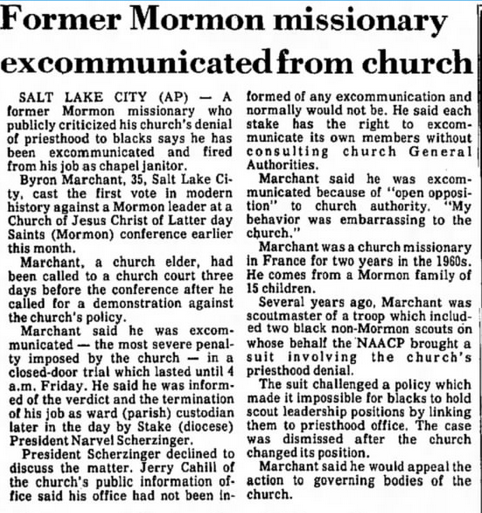
\includegraphics[width=0.4\linewidth]{articles/images/ex.png}
  \caption{The Daily Reporter (Dover, Ohio) 15 Oct 1977}
  \label{fig:ex1}
\end{figure}

In the early days of the church, leaders were known to excommunicate followers more
often and loose. It has slowed down a bit as church goers have gotten in line as it
were. But there are still excommunications which happen every year. Of course, not 
all end up in the newspaper like Figure \ref{fig:ex1}. But it still happens.

It was said during the succession crisis of 1844 after Joseph Smith died, anyone who
voted against Brigham Young were excommunicated. Even though a vote for and against
was called for. Anytime a person in the church votes against or opposing the leadders
of the church, they are in danger of apostasy.

To face excommunication from the church, you are taken off the roles of the church.
Your baptism becomes null and void, any temple blessings are revoked. You are not
able to speak in a church meeting, give a prayer, take the sacrament or participate
in any way at all.

Some people are shunned by their family members. This is not a church teaching to be
shunned, but it does happen. Family can't accept that one would not want to follow a
church they grew up in. They cannot understand how a person would abandon their God
as it were.

I think that's a main issue poeple don't understand. Just because a person is
excommunicated from the church, it doesn't mean they have lost faith in Christ and a
belief in God. Perhaps they have come to understand Christ a little bit more than
they did when in the LDS faith.

The leaders say it's to help the repentence process, to help others come back to the
church and to accept Christ's atonement in their lives. In effect, the church will
not leave them alone. If a person is openly opposing church leaders, maybe they want
to be left alone. It's a thought.

Members ask all the time to be left alone from the church, yet because the member is
on the role the church continues to visit the member. The only way to avoid any of
this is to either be excommunicated or to request your name be removed from the
records of the church.

Even removing your name isn't an easy process. The bishop of the local ward will
still want to see if there's anything they can do to help you come back to the fold.
It's a never ending process which constantly loops over again.

It's sad to think about.